\documentclass[11pt,compress,t,notes=noshow, xcolor=table]{beamer}
\usepackage[]{graphicx}\usepackage[]{color}
% maxwidth is the original width if it is less than linewidth
% otherwise use linewidth (to make sure the graphics do not exceed the margin)
\makeatletter
\def\maxwidth{ %
  \ifdim\Gin@nat@width>\linewidth
    \linewidth
  \else
    \Gin@nat@width
  \fi
}
\makeatother

\newcommand{\citebutton}[2]{%
\beamergotobutton{\href{#2}{#1}}%
}

\newcommand{\blu}[1]{\textcolor{blue}{#1}}
\newcommand{\org}[1]{\textcolor{orange}{#1}}
\newcommand{\ques}{\textbf{\textcolor{red}{Question:  }}}
\newcommand{\questionssofar}{\begin{frame}\frametitle{Any questions?}\end{frame}}

\newcommand\warning{%
 \makebox[1.4em][c]{%
 \makebox[0pt][c]{\raisebox{.1em}{\scriptsize!}}%
 \makebox[0pt][c]{\color{red}\normalsize$\bigtriangleup$}}}%

\definecolor{fgcolor}{rgb}{0.345, 0.345, 0.345}
\newcommand{\hlnum}[1]{\textcolor[rgb]{0.686,0.059,0.569}{#1}}%
\newcommand{\hlstr}[1]{\textcolor[rgb]{0.192,0.494,0.8}{#1}}%
\newcommand{\hlcom}[1]{\textcolor[rgb]{0.678,0.584,0.686}{\textit{#1}}}%
\newcommand{\hlopt}[1]{\textcolor[rgb]{0,0,0}{#1}}%
\newcommand{\hlstd}[1]{\textcolor[rgb]{0.345,0.345,0.345}{#1}}%
\newcommand{\hlkwa}[1]{\textcolor[rgb]{0.161,0.373,0.58}{\textbf{#1}}}%
\newcommand{\hlkwb}[1]{\textcolor[rgb]{0.69,0.353,0.396}{#1}}%
\newcommand{\hlkwc}[1]{\textcolor[rgb]{0.333,0.667,0.333}{#1}}%
\newcommand{\hlkwd}[1]{\textcolor[rgb]{0.737,0.353,0.396}{\textbf{#1}}}%
\let\hlipl\hlkwb

\usepackage{framed}
\makeatletter
\newenvironment{kframe}{%
 \def\at@end@of@kframe{}%
 \ifinner\ifhmode%
  \def\at@end@of@kframe{\end{minipage}}%
  \begin{minipage}{\columnwidth}%
 \fi\fi%
 \def\FrameCommand##1{\hskip\@totalleftmargin \hskip-\fboxsep
 \colorbox{shadecolor}{##1}\hskip-\fboxsep
     % There is no \\@totalrightmargin, so:
     \hskip-\linewidth \hskip-\@totalleftmargin \hskip\columnwidth}%
 \MakeFramed {\advance\hsize-\width
   \@totalleftmargin\z@ \linewidth\hsize
   \@setminipage}}%
 {\par\unskip\endMakeFramed%
 \at@end@of@kframe}
\makeatother

\definecolor{shadecolor}{rgb}{.97, .97, .97}
\definecolor{messagecolor}{rgb}{0, 0, 0}
\definecolor{warningcolor}{rgb}{1, 0, 1}
\definecolor{errorcolor}{rgb}{1, 0, 0}
\newenvironment{knitrout}{}{} % an empty environment to be redefined in TeX

\usepackage{alltt}
\newcommand{\SweaveOpts}[1]{}  % do not interfere with LaTeX
\newcommand{\SweaveInput}[1]{} % because they are not real TeX commands
\newcommand{\Sexpr}[1]{}       % will only be parsed by R
\newcommand{\xmark}{\ding{55}}%


\usepackage[english]{babel}
\usepackage[utf8]{inputenc}

\usepackage{dsfont}
\usepackage{verbatim}
\usepackage{amsmath}
\usepackage{amsfonts}
\usepackage{amssymb}
\usepackage{bm}
\usepackage{csquotes}
\usepackage{multirow}
\usepackage{longtable}
\usepackage{booktabs}
\usepackage{enumerate}
\usepackage[absolute,overlay]{textpos}
\usepackage{psfrag}
\usepackage{algorithm}
\usepackage{algpseudocode}
\usepackage{eqnarray}
\usepackage{arydshln}
\usepackage{tabularx}
\usepackage{placeins}
\usepackage{tikz}
\usepackage{setspace}
\usepackage{colortbl}
\usepackage{mathtools}
\usepackage{wrapfig}
\usepackage{bm}
\usepackage{amsmath}
\usepackage{pifont}

\usetikzlibrary{shapes.multipart,shapes,arrows,automata,positioning,calc,chains,trees, shadows}
\tikzset{
  %Define standard arrow tip
  >=stealth',
  %Define style for boxes
  punkt/.style={
    rectangle,
    rounded corners,
    draw=black, very thick,
    text width=6.5em,
    minimum height=2em,
    text centered},
  % Define arrow style
  pil/.style={
    ->,
    thick,
    shorten <=2pt,
    shorten >=2pt,}
}

\tikzstyle{vec}=[draw, rectangle, fill = white, minimum width=5mm, minimum height=1cm, inner sep = 2pt]

\usepackage{subfig}

% Defines macros and environments
\usepackage{../../style/lmu-lecture}


\let\code=\texttt
\let\proglang=\textsf

\setkeys{Gin}{width=0.9\textwidth}

\setbeamertemplate{frametitle}{\expandafter\uppercase\expandafter\insertframetitle}

\usepackage{bbm}
% basic latex stuff
\newcommand{\pkg}[1]{{\fontseries{b}\selectfont #1}} %fontstyle for R packages
\newcommand{\lz}{\vspace{0.5cm}} %vertical space
\newcommand{\dlz}{\vspace{1cm}} %double vertical space
\newcommand{\oneliner}[1] % Oneliner for important statements
{\begin{block}{}\begin{center}\begin{Large}#1\end{Large}\end{center}\end{block}}


%new environments
\newenvironment{vbframe}  %frame with breaks and verbatim
{
 \begin{frame}[containsverbatim,allowframebreaks]
}
{
\end{frame}
}

\newenvironment{vframe}  %frame with verbatim without breaks (to avoid numbering one slided frames)
{
 \begin{frame}[containsverbatim]
}
{
\end{frame}
}

\newenvironment{blocki}[1]   % itemize block
{
 \begin{block}{#1}\begin{itemize}
}
{
\end{itemize}\end{block}
}

\newenvironment{fragileframe}[2]{  %fragile frame with framebreaks
\begin{frame}[allowframebreaks, fragile, environment = fragileframe]
\frametitle{#1}
#2}
{\end{frame}}


\newcommand{\myframe}[2]{  %short for frame with framebreaks
\begin{frame}[allowframebreaks]
\frametitle{#1}
#2
\end{frame}}

\newcommand{\remark}[1]{
  \textbf{Remark:} #1
}


\newenvironment{deleteframe}
{
\begingroup
\usebackgroundtemplate{
\includegraphics[width=\paperwidth,height=\paperheight]{../style/color/red.png}}
 \begin{frame}
}
{
\end{frame}
\endgroup
}
\newenvironment{simplifyframe}
{
\begingroup
\usebackgroundtemplate{
\includegraphics[width=\paperwidth,height=\paperheight]{../style/color/yellow.png}}
 \begin{frame}
}
{
\end{frame}
\endgroup
}\newenvironment{draftframe}
{
\begingroup
\usebackgroundtemplate{
\includegraphics[width=\paperwidth,height=\paperheight]{../style/color/green.jpg}}
 \begin{frame}
}
{
\end{frame}
\endgroup
}
% https://tex.stackexchange.com/a/261480: textcolor that works in mathmode
\makeatletter
\renewcommand*{\@textcolor}[3]{%
  \protect\leavevmode
  \begingroup
    \color#1{#2}#3%
  \endgroup
}
\makeatother





\input{../../latex-math/basic-math.tex}
\input{../../latex-math/basic-ml.tex}

\newcommand{\titlefigure}{figure/tokenization.jpeg}
\newcommand{\learninggoals}{
\item Understand the the process of text tokenization
\item Learn the various types of text tokenization}

\title{Deep Learning Basics}
% \author{}
\institute{\href{https://slds-lmu.github.io/lecture_dl4nlp/}{slds-lmu.github.io/lecture\_dl4nlp}}
\date{}

\begin{document}
\lecturechapter{Revisiting words: Tokenization}
\lecture{Deep Learning for NLP}

% ------------------------------------------------------------------------------

\begin{vbframe}{Process of Text Tokenization}

\vfill

\begin{itemize}
	\item Breaking text into smaller units called tokens
		\begin{itemize}
			\item Tokens are discrete text units (letters, words, etc.)
			\item They are the building blocks of natural language
		\end{itemize}
	\item Encoding each token with unique IDs (numbers)
	\item Performed on the entire corpus of documents
		\begin{itemize}
			\item Corpus vocabulary of unique tokens is obtained
		\end{itemize}
	\item Mandatory preprocessing step for most of NLP tasks

\end{itemize}

\vfill

\end{vbframe}

% ------------------------------------------------------------------------------

\begin{vbframe}{Why Tokenize?}

\vfill

\begin{itemize}
	\item Computers must understand text
		\begin{itemize}
			\item Text encoding is necessary
			\item Encode small rather than large units
		\end{itemize}
	\item Corpus documents can be large and hard to interpret
		\begin{itemize}
			\item Working with tokens is easier
			\item Building meaning in bottom-up fashion
		\end{itemize}
	\item Text may contain extra whitespaces
		\begin{itemize}
			\item Tokenization removes them
		\end{itemize}
\end{itemize}

\vfill

\end{vbframe}

% ------------------------------------------------------------------------------

\begin{vbframe}{Tokenization in action}

\vfill

	\begin{figure}
		\centering
		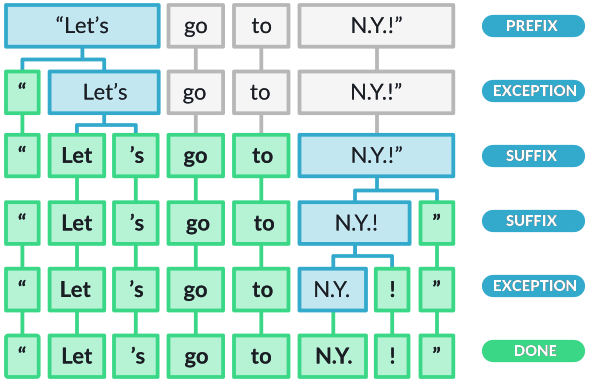
\includegraphics[width = 9cm]{figure/spacy_tok}\\ 
		\footnotesize{Source:} \href{https://spacy.io/usage/linguistic-features}{\footnotesize \it spaCy}
	\end{figure}

\vfill

\end{vbframe}

% ------------------------------------------------------------------------------

\begin{vbframe}{Tokenization Types}

\vfill

\begin{itemize}
	\item Paragraph tokenization 
		\begin{itemize}
			\item Breaking doucments in paragraphs 
			\item Rarely used
		\end{itemize}
		\item Sentence tokenization 
			\begin{itemize}
				\item Breaking text in sentences 
			\end{itemize}
		\item Word tokenization
			\begin{itemize}
				\item Breaking text in words
				\item The most common
			\end{itemize}
	\item Subword tokenization
		\begin{itemize}
			\item Breaking words in morphemes
		\end{itemize}
	\item Character tokenization
		\begin{itemize}
			\item Breaking text in individual characters
		\end{itemize}
	\item Whitespace tokenization
		\begin{itemize}
			\item Typical whitespaces: \verb|" ", \t, \n|
		\end{itemize}
\end{itemize}

\vfill

\end{vbframe}

% ------------------------------------------------------------------------------

\begin{vbframe}{Word Tokenization}

\vfill

\begin{itemize}
	\item Most popular type of tokenization
		\begin{itemize}
			\item Applied as preprocessing step in most NLP tasks
		\end{itemize}
	\item Considers dictionary words and several delimiters
		\begin{itemize}
			\item Accuracy depends on dictionary used for training
			\item Tradeoff between accuracy and efficiency
		\end{itemize}
	\item Whitespaces and punctuation symbols are used 
		\begin{itemize}
			\item They determine word boundaries
		\end{itemize}
	\item Available in many NLP libraries
\end{itemize}

\vskip5mm
Example: \vskip3mm 
{\small\it What is the tallest building? => `What', `is', `the', `tallest', `building', `?'}

\vfill

\end{vbframe}

% ------------------------------------------------------------------------------

\begin{vbframe}{Subword Tokenization}

\vfill

\begin{itemize}
	\item Finer grained than word tokenization
		\begin{itemize}
			\item Breaks text into words
			\item Breaks words into smaller units (root, prefix, suffix, etc.)
			\item Uses more complex linguistic rules
		\end{itemize}
	\item More important for highly flective languages
		\begin{itemize}
			\item Words have many forms
			\item Prefixes and suffixes are added
			\item Word meaning and function changes
		\end{itemize}
	\item Helps to disambiguate meaning 
	\item Helps to reduce out of vocabulary words
\end{itemize}

\vskip5mm
Example: \vskip3mm 
{\small\it What is the tallest building? => `What', `is', `the', `tall', `est', `build', `ing', `?'}

\vfill

\end{vbframe}

% ------------------------------------------------------------------------------

\begin{vbframe}{Character Tokenization}

\vfill

\begin{itemize}
	\item Creates smaller vocabulary
		\begin{itemize}
			\item Same as the number of lettters
		\end{itemize}
	\item Helps with out of vocabulary words
		\begin{itemize}
			\item Retains their character composition
		\end{itemize}
	\item More complex process
		\begin{itemize}
			\item The output becomes 5 or 6 times bigger
		\end{itemize}
\end{itemize}

\vskip5mm
Example: \vskip3mm 
{\small\it What is the tallest building? => `W', `h', `a', `t', `i', `s', `t', `h', `e', `t', `a', `l', `l', `e', `s', `t', `b', `u', `i', `l', `d', `i', `n', `g', `?'}

\vfill

\end{vbframe}

% ------------------------------------------------------------------------------

\begin{vbframe}{Remember FastText?}

\vfill

\textbf{Assume, we want to represent the word \textit{example}:}

\begin{itemize}
	\item Character n-grams (n = 3):  
		$$\text{<ex, exa, xam, amp, mpl, ple, le>, <example>}$$
	\item In practice, we don't set $n = a$ but rather $a \leq n \leq b$
	\item Character n-grams ($2 \leq n \leq 4$):
  \begin{align*}
    & \text{<e, ex, xa, am, mp, pl, le, e>,} \\
    & \text{<ex, exa, xam, amp, mpl, ple, le>,} \\
    & \text{<exa, exam, xamp, ampl, mple, ple>,} \\
		& \text{<example>}
  \end{align*}
	\item Note, that the 4-gram \textit{exam} is different from the word $<$exam$>$.
\end{itemize}

\vfill

\end{vbframe}

% ------------------------------------------------------------------------------

\begin{vbframe}{BytePair encoding (BPE)}

\vfill

\textbf{Data compression algorithm \href{https://www.derczynski.com/papers/archive/BPE_Gage.pdf}{\beamergotobutton{Gage (1994)}}}

	\begin{itemize}
		\item Considering data on a \textit{byte}-level
		\item Looking at pairs of bytes:
			\begin{enumerate}
				\item Count the occurrences of all byte pairs
				\item Find the most frequent byte pair
				\item Replace it with an unused byte
			\end{enumerate}
		\item Repeat this process until no further compression is possible
	\end{itemize}

\vfill

\end{vbframe}

% ------------------------------------------------------------------------------

\begin{vbframe}{BytePair encoding (BPE)}

\vfill

\textbf{Open-vocabulary neural machine translation \href{https://www.aclweb.org/anthology/P16-1162.pdf}{\beamergotobutton{Sennrich et al. (2016)}}}
	
	\begin{itemize}
		\item Instead of looking at bytes, look at characters
		\item Motivation: Translation as an open-vocabulary problem
		\item Word-level NMT models:
			\begin{itemize}
				\item Handling out-of-vocabulary word by using back-off dictionaries
				\item Unable to translate or generate previously unseen words
			\end{itemize}
		\item Using BPE effectively \textit{solves} this problem, except for ..
			\begin{itemize}
				\item .. the occurence of unknown characters
				\item .. when all occurences in the training set were merged into "larger" symbols
							(Example: \textit{"safeguar"} and \textit{"safeguard"})
			\end{itemize}
	\end{itemize}

\vfill

\end{vbframe}

% ------------------------------------------------------------------------------

\begin{vbframe}{BytePair encoding (BPE)}

\vfill

\textbf{Adapt BPE for word segmentation \href{https://www.aclweb.org/anthology/P16-1162.pdf}{\beamergotobutton{Sennrich et al. (2016)}}}

	\begin{itemize}
		\item \textit{Goal:} Represent an open vocabulary by a vocabulary of fixed size\\
					$\rightarrow$ Use variable-length character sequences 
		\item Looking at pairs of characters:
			\begin{enumerate}
				\item Initialize the the vocabulary with all characters plus end-of-word token
				\item Count occurrences and find the most frequent character pair,\\
							e.g. "A" and "B" (\warning Word boundaries are \textbf{not} crossed) \\
							\textit{[Side effect: Can be run on a dictionary w/ frequency counts]}
				\item Replace it with the new token "AB"
			\end{enumerate}
		\item Only one hyperparameter: Vocabulary size\\
					(Initial vocabulary + Specified no. of merge operations)\\
					$\rightarrow$ Repeat this process until given $|V|$ is reached
	\end{itemize}

\vfill

\end{vbframe}

% ------------------------------------------------------------------------------

\begin{vbframe}{Example -- Setup}

\begin{lstlisting}[language=Python]
import re, collections

def get_stats(vocab):
  pairs = collections.defaultdict(int)
  for word, freq in vocab.items():
    symbols = word.split()
    for i in range(len(symbols)-1):
      pairs[symbols[i],symbols[i+1]] += freq
  return pairs
	
def merge_vocab(pair, v_in):
  v_out = {}
  bigram = re.escape(' '.join(pair))
  p = re.compile(r'(?<!\S)' + bigram + r'(?!\S)')
  for word in v_in:
    w_out = p.sub(''.join(pair), word)
    v_out[w_out] = v_in[word]
  return v_out
\end{lstlisting}

\end{vbframe}

% ------------------------------------------------------------------------------

\begin{vbframe}{Example -- Merging}

\vspace{-.5cm}

\begin{lstlisting}[language=Python]
vocab = {'l o w </w>' : 5, 'l o w e r </w>' : 2, 
				 'n e w e s t </w>':6, 'w i d e s t </w>':3}

pairs = get_stats(vocab)
\end{lstlisting}

\vspace{-.75cm}

\begin{lstlisting}[language=Python]
>>> print(pairs)
defaultdict(<class 'int'>, {
						('l', 'o'): 7, ('o', 'w'): 7, ('w', '</w>'): 5, 
						('w', 'e'): 8, ('e', 'r'): 2, ('r', '</w>'): 2, 
						('n', 'e'): 6, ('e', 'w'): 6, ('e', 's'): 9, 
						('s', 't'): 9, ('t', '</w>'): 9, ('w', 'i'): 3, 
						('i', 'd'): 3, ('d', 'e'): 3
})
\end{lstlisting}

\vspace{-.5cm}

\begin{lstlisting}[language=Python]
best = max(pairs, key=pairs.get)
vocab = merge_vocab(best, vocab)
\end{lstlisting}

\vspace{-.75cm}

\begin{lstlisting}[language=Python]
>>> print(best)
('e', 's')
>>> print(vocab)
{'l o w </w>': 5, 'l o w e r </w>': 2, 
 'n e w es t </w>': 6, 'w i d es t </w>': 3}
\end{lstlisting}

\end{vbframe}

% ------------------------------------------------------------------------------

\begin{vbframe}{Example -- Merging}

\vspace{-.5cm}

\begin{lstlisting}[language=Python]
vocab = {'l o w </w>' : 5, 'l o w e r </w>' : 2, 
				 'n e w e s t </w>':6, 'w i d e s t </w>':3}

num_merges = 10

for i in range(num_merges):
  pairs = get_stats(vocab)
  best = max(pairs, key=pairs.get)
  vocab = merge_vocab(best, vocab)
  print(best)
\end{lstlisting}

\vspace{-.5cm}

\begin{lstlisting}[language=Python]
('e', 's')
('es', 't')
('est', '</w>')
('l', 'o')
('lo', 'w')
('n', 'e')
('ne', 'w')
('new', 'est</w>')
('low', '</w>')
('w', 'i')
\end{lstlisting}

\end{vbframe}

% ------------------------------------------------------------------------------

\begin{frame}{WordPiece}

\vfill

	\textbf{Voice Search for Japanese and Korean \href{https://storage.googleapis.com/pub-tools-public-publication-data/pdf/37842.pdf}{\beamergotobutton{Schuster \& Nakajima (2012)}}}

	\begin{itemize}
		\item \textit{Specific Problems:} 
			\begin{itemize}
				\item Asian languages have larger basic character inventories compared to Western languages
				\item Concept of spaces between words does (partly) not exist
				\item Many different pronounciations for each character
			\end{itemize}
	\end{itemize}
	
\vfill

\end{frame}

% ------------------------------------------------------------------------------

\begin{frame}{WordPiece}

\vfill

	\begin{itemize}
		\item \textit{WordPieceModel:} Data-dependent + do not produce OOVs
			\begin{enumerate}
				\item Initialize the the vocabulary with basic Unicode characters (22k for Japanese, 11k for Korean)\\
							\warning Spaces are indicated by an underscore attached before (of after) the respective basic unit or word (increases initial $|V|$ by up to factor 4)
				\item Build a language model using this vocabulary
				\item Merge word units that increase the likelihood on the training data the most, when added to the model
			\end{enumerate}
		\item Two possible stopping criteria:\\Vocabulary size \textit{or} incremental increase of the likelihood
	\end{itemize}
	
\vfill

\end{frame}

% ------------------------------------------------------------------------------

\begin{frame}{WordPiece}

\vfill

	\textbf{Use for neural machine translation \href{https://arxiv.org/pdf/1609.08144.pdf}{\beamergotobutton{Wu et al. (2016)}}}

	\begin{itemize}
		\item \textit{Adaptions:} 
			\begin{itemize}
				\item Application to Western languages leads to a lower number of basic units ($\sim$ 500)
				\item Add space markers (underscores) \textit{only} at the beginning of words
				\item Final vocabulary sizes between 8k and 32k yield a good balance between accuracy and fast decoding speed\\(compared to around 200k from \href{https://storage.googleapis.com/pub-tools-public-publication-data/pdf/37842.pdf}{\beamergotobutton{Schuster \& Nakajima (2012)}})
			\end{itemize}
	\end{itemize}
	
	\vspace{.3cm}
	
	\textit{Independent} \textbf{vs.} \textit{joint} \textbf{encodings for source \& target language}
	
	\begin{itemize}
		\item Sennrich et al. (2016) report better results for joint BPE
		\item Wu et al. (2016) use shared WordPieceModel to guarantee identical segmentation in source \& target language in order to facilitate copying rare entity names or numbers
	\end{itemize}
	
\vfill

\end{frame}

% ------------------------------------------------------------------------------

\endlecture
\end{document}
